\documentclass[letter, 10pt]{article}
\usepackage{fullpage}
\usepackage[margin=0.4in]{geometry}
\usepackage{graphicx}
\usepackage{caption}
\usepackage{subcaption}
\usepackage{amsmath}
\usepackage{listings}
\usepackage{float}
\usepackage{array,multirow}
\usepackage{tikz}
\usepackage{cancel}
\setcounter{MaxMatrixCols}{20}
\usetikzlibrary{arrows}
\pagenumbering{gobble}
\begin{document}
\noindent
\large \textbf{Rahul Ghosh} \hfill \textbf{Assignment\#3}\\
\normalsize Student ID: 5476965 \hfill CSci 5512\\

\section*{Question 1}
If we represent the Bayesian Network with matrices:
\begin{equation*}
    P(x_0) = 
    \begin{bmatrix}
        1/3\\
        1/3\\
        1/3
    \end{bmatrix}
    \quad
    P(x_{t+1}|x_t) = T =
    \begin{bmatrix}
        0.6 & 0.35 & 0.05 \\
        0.2 & 0.6 & 0.2 \\
        0 & 0.5 & 0.5
    \end{bmatrix}
    \quad
    P(e_t|x_t) = E_t =
    \begin{bmatrix}
        0 & 0 & 0 \\
        0 & 0.05 & 0 \\
        0 & 0 & 0.4
    \end{bmatrix}
    \quad
    P(\neg e_t|x_t) = E_t =
    \begin{bmatrix}
        1 & 0 & 0 \\
        0 & 0.95 & 0 \\
        0 & 0 & 0.6
    \end{bmatrix}
\end{equation*}
The filtering equation can be written with matrices as:
\begin{equation*}
    F_{t+1} = \alpha E_{t+1}T'F_t, \quad where\ F_0 = P(x_0)
\end{equation*}
\begin{itemize}
    \item[(1)] $P(x_1|e_1=``not flooded") = P(x_1| \neg e_1) = F_1 = \alpha E_1T'F_0 = 
    \begin{bmatrix}
        0.304472\\
        0.524263\\
        0.171265
    \end{bmatrix}$
    \item[(2)] $P(x_2|e_1=``not flooded", e_2=``not flooded") = P(x_2|\neg e_1, \neg e_2) = F_2 = \alpha E_2T'F_1 = 
    \begin{bmatrix}
        0.322213\\
        0.539477\\
        0.13831
    \end{bmatrix}$
    \item[(2)] $P(x_3|e_1=``not flooded", e_2=``not flooded", e_3=``flooded") = P(x_3| \neg e_1, \neg e_2, e_3) = F_1 = \alpha E_3T'F_2 = 
    \begin{bmatrix}
        0\\
        0.246533\\
        0.753467
    \end{bmatrix}$
\end{itemize}
The values are for low, med and high respectively.
\section*{Question 2} The filtering equation can be written with matrices as:
\begin{equation*}
    B_t = TE_{t+1}B_{t+1}, \quad where\ B_T = \begin{bmatrix}1\\1\\1\end{bmatrix}
\end{equation*}
Thus the smoothing equation is given as 
\begin{equation*}
    S_t = \alpha F_t B_t
\end{equation*}
\begin{itemize}
    \item[(1)] $P(x_1|e_1=``not flooded", e_2=``not flooded", e_3=``flooded") = P(x_1| \neg e_1, \neg e_2, e_3) = S_1 = \alpha F_1B_1 = 
    \begin{bmatrix}
        0.219015\\
        0.556865\\
        0.22412
    \end{bmatrix}$
    \item[(2)] $P(x_2|e_1=``not flooded", e_2=``not flooded", e_3=``flooded") = P(x_2| \neg e_1, \neg e_2, e_3) = S_2 = \alpha F_2B_2 = 
    \begin{bmatrix}
        0.117831\\
        0.578695\\
        0.303474
    \end{bmatrix}$
    \item[(2)] $P(x_3|e_1=``not flooded", e_2=``not flooded", e_3=``flooded") = P(x_3| \neg e_1, \neg e_2, e_3) = S_3 = \alpha F_3B_3 = 
    \begin{bmatrix}
        0\\
        0.246533\\
        0.753467
    \end{bmatrix}$
\end{itemize}
\begin{figure}[H]
    \minipage{0.33\textwidth}
        \centering
        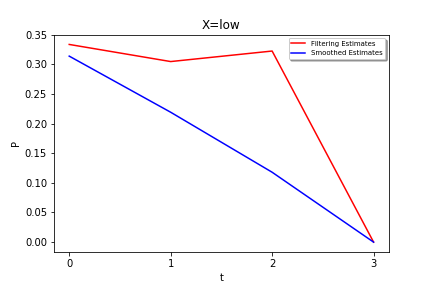
\includegraphics[width=\textwidth]{HW3/low.png}
    \endminipage\hfill
    \minipage{0.33\textwidth}
        \centering
        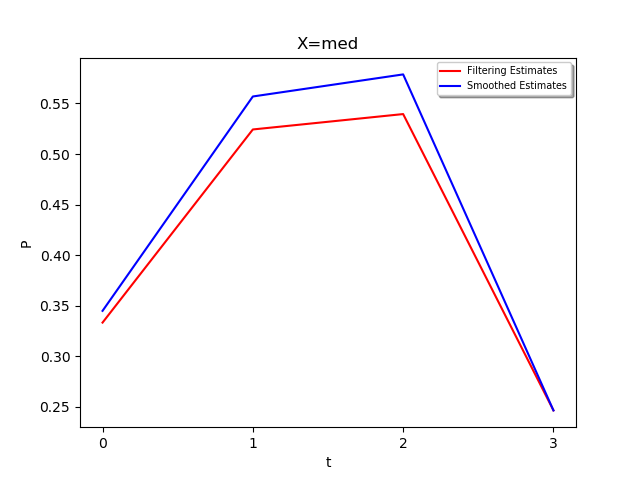
\includegraphics[width=\textwidth]{HW3/med.png}
    \endminipage\hfill
    \minipage{0.33\textwidth}
        \centering
        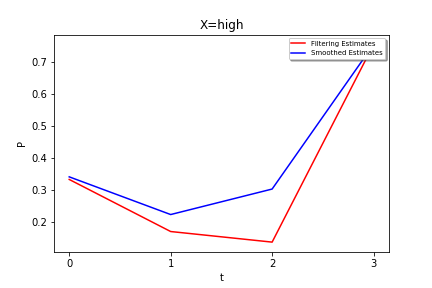
\includegraphics[width=\textwidth]{HW3/high.png}
    \endminipage\hfill
    \caption{Probability of filtered and smoothed estimates}
\end{figure}
\section*{Question 3}
If we represent the Bayesian Network with matrices:
\begin{equation*}
    P(x_0) = 
    \begin{bmatrix}
        1/3\\
        1/3\\
        1/3
    \end{bmatrix}
    \quad
    P(x_{t+1}|x_t) = T =
    \begin{bmatrix}
        0.6 & 0.35 & 0.05 \\
        0.2 & 0.6 & 0.2 \\
        0 & 0.5 & 0.5
    \end{bmatrix}
    \quad
    P(e_t|x_t) = E_t =
    \begin{bmatrix}
        0 & 1\\
        0.05 & 0.95 \\
        0.4 & 0.6
    \end{bmatrix}
\end{equation*}
Using the matrices we create the MLE table using the following equation
\begin{equation*}
    MLE(t+1) = P(e_t|x_t)\max_{x_t} P(x_{t+1}|x_t) MLE(t)
\end{equation*}
For the given evidence: $e_1=“flooded”, e_2=“not flooded”, e_3=“not flooded”, e_4=“flooded”, e_5=“not flooded”$, we get the table as,
\begin{equation*}
    MLE = 
    \begin{bmatrix}
    0.333333333 & 0 & 0.002 & 0.00633333333 & 0 & 0.0001083\\
    0.333333333 & 0.01 & 0.0316666667 & 0.01805 & 0.0005415 & 0.0006859\\
    0.333333333 & 0.0666666667 & 0.02 & 0.006 & 0.001444 & 0.0004332
    \end{bmatrix}
\end{equation*}
Thus the sequence we get is $[x_0=low, x_1=high, x_2=med, x_3=med, x_4=high, x_5=med]$\\
For the given evidence: $e_1=“flooded”, e_2=“not flooded”, e_3=“not flooded”, e_4=“flooded”, e_5=“not flooded”, e_6="flooded"$, we get the table as,
\begin{equation*}
    MLE = 
    \begin{bmatrix}
    0.333333333 & 0 & 0.002 & 0.00633333333 & 0 & 0.0001083 & 0\\
    0.333333333 & 0.01 & 0.0316666667 & 0.01805 & 0.0005415 & 0.0006859 & 0.000020577\\
    0.333333333 & 0.0666666667 & 0.02 & 0.006 & 0.001444 & 0.0004332 & 0.00008664
    \end{bmatrix}
\end{equation*}
Thus the sequence we get is $[x_0=low, x_1=high, x_2=med, x_3=med, x_4=high, x_5=med, x_6=high]$\\
\section*{Question 4}Using N=100 particles and the particle filtering algorithm, we get the following distribution of particles,
\begin{equation*}
    \begin{bmatrix}
    38 & 19 & 24 & 0 & 0 & 1 & 19 & 31 & 21 & 0 & 4\\
    29 & 55 & 56 & 28 & 19 & 68 & 54 & 49 & 57 & 14 & 51\\
    33 & 26 & 20 & 72 & 81 & 31 & 27 & 20 & 22 & 86 & 45
    \end{bmatrix}
\end{equation*}
Therefore, $P(x_{10}|\neg e_1, \neg e_2, e_3, e_4, \neg e_5, \neg e_6, \neg e_7, \neg e_8, e_9) = \begin{bmatrix}0\\0.51\\0.49\end{bmatrix}$
\section*{Question 5}
$P(x_0) = \mathcal{N}(0,1) \implies \sigma_0^2=1$\\
$P(e_t|x_t) = \mathcal{N}(x_t,0.75) \implies \sigma_z^2=0.75$\\
The accuracy of our throw is $\sigma_x^2$\\
The variance at time t+1 is given by $\sigma_{t+1}^2 = \frac{(\sigma_t^2 + \sigma_x^2)\sigma_z^2}{\sigma_t^2 + \sigma_x^2 + \sigma_z^2}$
For 

\begin{figure}[H]
    \centering
        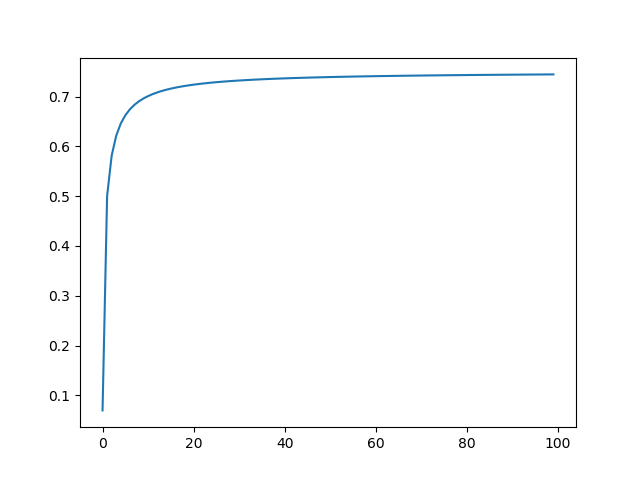
\includegraphics[width=\textwidth]{HW3/variance.png}
    \caption{Probability of filtered and smoothed estimates}
\end{figure}

\section*{Question 6}
\end{document}